\chapter{\Large Iteración III: “Priorización de alertas”}
    El objetivo de asignar distintos niveles de prioridad a las alertas generadas por los eventos que suceden, radica en la naturaleza de estos últimos, su importancia y la gestión de la atención de los analistas del CSIRT. Esto se debe a las necesidades de optimizar el uso de los recursos técnicos y humanos del centro de respuesta a incidentes para cumplir de la manera más eficiente posible con los objetivos y políticas de la organización a la cual pertenece. \par
    De esta manera, la naturaleza de los incidentes determina su elegibilidad para una respuesta automatizada al tener en cuenta por un lado su estructura bien conocida y por el otro su alta tasa de repetición en un periodo determinado. En estos casos, sería inútil destinar valiosos recursos tales como la atención de un analista que ya conoce perfectamente la estructura de este tipo de eventos y por lo tanto la respuesta apropiada a él. También se incluyen aquellos casos en los que aún conocida su estructura, el incidente proviene en simultáneo de múltiples fuentes en muy poco tiempo, de manera que la capacidad humana de responder de a un evento a la vez resulta sobrepasada y por lo tanto, ineficiente. Estos son los casos de ataques de reconocimiento y los de denegación distribuida de servicio (DDoS), entre otros. \par
    La solución a esta situación se encontró, en primer lugar, en otorgar una baja prioridad a las alertas que estos eventos generaban. Luego se adaptó el sistema de notificaciones para evitar que estas hubiesen abrumado a los analistas y responsables de los activos de información. Finalmente, se consideró la automatización de respuestas a estos incidentes en los casos viables. \par
    \begin{section}{Reglas y prioridades}
    En Security Onion y otros sistemas, el elemento descriptor que identifica y procesa a cada definición de incidente es la regla. Las reglas comprenden una serie de campos que describen con precisión la naturaleza de un incidente dado y por lo tanto, existen tantas reglas como amenazas detectadas en circulación. \par
    Cuando un nuevo malware es descubierto por el equipo de algún CSIRT con la suficiente capacidad de investigación o reportado a un laboratorio apropiado para este fin, es posible realizar un estudio de sus características y una vez identificadas estas últimas, proceder a crear una regla. Esta ultima es agregada al repositorio correspondiente para que otros CSIRT actualicen sus IDS con esta nueva definición y así contar con un filtro (la regla) que permita detectar este malware. Las reglas tienen un conjunto de campos donde se detallan características del paquete y su contexto, tales como el puerto de origen y destino, protocolo empleado, dirección IP, etc y unos campos dedicados a la naturaleza del incidente (clasificación, mensaje, prioridad, etc). Algunos de estos campos son comunes a todas las reglas y permiten agruparlas para administrar eficientemente las alertas generadas cuando una regla coincide con la descripción de un incidente. Dado que estos campos también se pueden considerar \textit{observables}, es posible utilizarlos en TheHive para gestionar incidentes y crear casos. \par
    Como se indicó anteriormente, la estructura de las reglas consisten en dos partes bien definidas: un encabezado (header) que es obligatorio  y un conjunto de campos opcionales. Dentro del header encontramos la acción (alerta, notificación, etc), el protocolo (tcp, udp), puertos de origen y destino, el sentido del evento (entrante o bidireccional) y las direcciones IP de origen y destino. \par
    La segunda parte de las reglas incluye dos tipos de campos: los que describen la naturaleza del evento y aquellos que contienen información del paquete de datos. Dentro del primer grupo encontramos aquellos tales como msg (descripción del evento), sid (id de la firma), classtype (clasificación de reglas o alertas), priority (prioridad de la firma y/o alerta), target (especifica de qué lado está el objetivo, es decir puerto de origen y puerto de destino), entre otros. El segundo grupo contiene datos extraídos que provienen desde de la capa de red hasta la capa de aplicación de la pila OSI. Se pueden mencionar a los campos “GeoIP” (localización geográfica de la IP), “Fragbits” (presencia del bit de fragmentación), “ACK” (presencia del campo ACK en paquete TCP), “itype” (número del tipo de mensaje ICMP), “http.method” (tipo de método HTTP usado), entre otros.
    \begin{figure}[H]
        \centering
        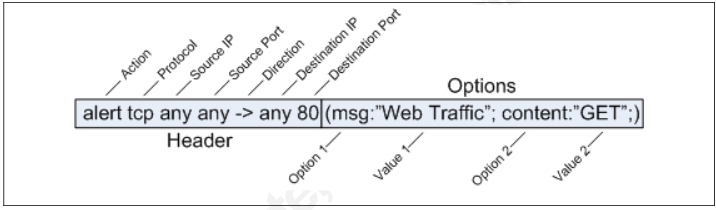
\includegraphics[width=0.7\textwidth]{./iteracion_3_imagenes/figura_41_estructura_regla.png}
        \caption{Estructura general de una regla}
        \label{fig:figura_41_estruc_regla}
    \end{figure}
    \FloatBarrier
    Como los campos están presentes en todas las reglas, es posible hacer uso de algunos de ellos para agrupar reglas que describen amenazas pertenecientes a un mismo grupo o categoría de malware: intentos de intrusión, reconocimiento, escalado de privilegios, etc y por lo tanto son útiles para gestionar los incidentes. \par
    Fue posible gestionar la configuración a través de un archivo que relaciona los siguientes campos: categorías de eventos y prioridades de la alerta generada. Este archivo llamado “\textit{classification.config}” se encuentra bajo el directorio que almacena las reglas descargadas desde diversas fuentes; en particular relaciona los campos “classtype” con “priority”, de manera tal que cualquier regla cuyo campo classtype contenga a los descritos en este archivo, generará una alerta con prioridad definida también en este ultimo. De esta manera, fue posible administrar un enorme número de reglas agrupadas en un reducido grupo de categorías y modificar el nivel de prioridad asociadas a ellas, esto tuvo impacto en las alertas que generaba el sistema. \par
    
    \begin{section}{Verificación de RF5: Definición de criterio para priorizar alertas.}
    
    Se dispuso de aproximadamente cuarenta y siete (47) categorías de incidentes disponibles por defecto, consideramos para el máximo nivel de prioridad a siete clasificaciones dado su nivel de ocurrencia y nivel de impacto para la organización. Las categorías a las que asignamos el máximo nivel de prioridad fueron las siguientes:
    \begin{itemize}
        \item Web-application-attack: esta categoría engloba a un conjunto enorme de malware y ataques a nivel de capa de aplicación. Gusanos, ransomware, ataques de reconocimiento entre otras amenazas comparten esta categoría. Sobre el caso particular de los ataques de reconocimiento, se aplicaron filtros para separarlos de los demás ya mencionados.
        \item Unsuccessful User: intentos repetidos de ganar acceso en ciertos activos e infraestructura de la organización.
        \item Attempted-dos: intentos de ataque de denegación de servicio y su variante distribuida
        \item Known client side exploit attempt: intento de ejecución de exploits en el lado del cliente.
        \item Exploit Kit Activity Detected: detección de actividad de un kit de exploits
        \item A suspicious filename was detected: detección de nombres de archivos sospechosos
        \item Network Trojan: detección de un virus troyano de red.
    \end{itemize}
    
    Para verificar el cumplimiento del requerimiento funcional 5, se procedió a editar el archivo  classification.config que se encuentra en el path /etc/nsm/rules/. En la Figura \ref{fig:squert-L2} se observa la detección de un incidente de reconocimiento en Squert. Este incidente pertenece a la categoría “attempted-recon” y en el archivo \textit{classification.config} esta categoría tiene un nivel de prioridad 2, tal como se muestra en la figura (barra vertical naranja). Esto se puede observar con más detalle al analizar los campos de la alerta en Kibana, como se muestra en la Figura \ref{fig:Kibana-L2}. Se remarcó el campo “priority”, donde se vio que efectivamente el valor de la prioridad es 2.
    \begin{figure}[H]
        \centering
        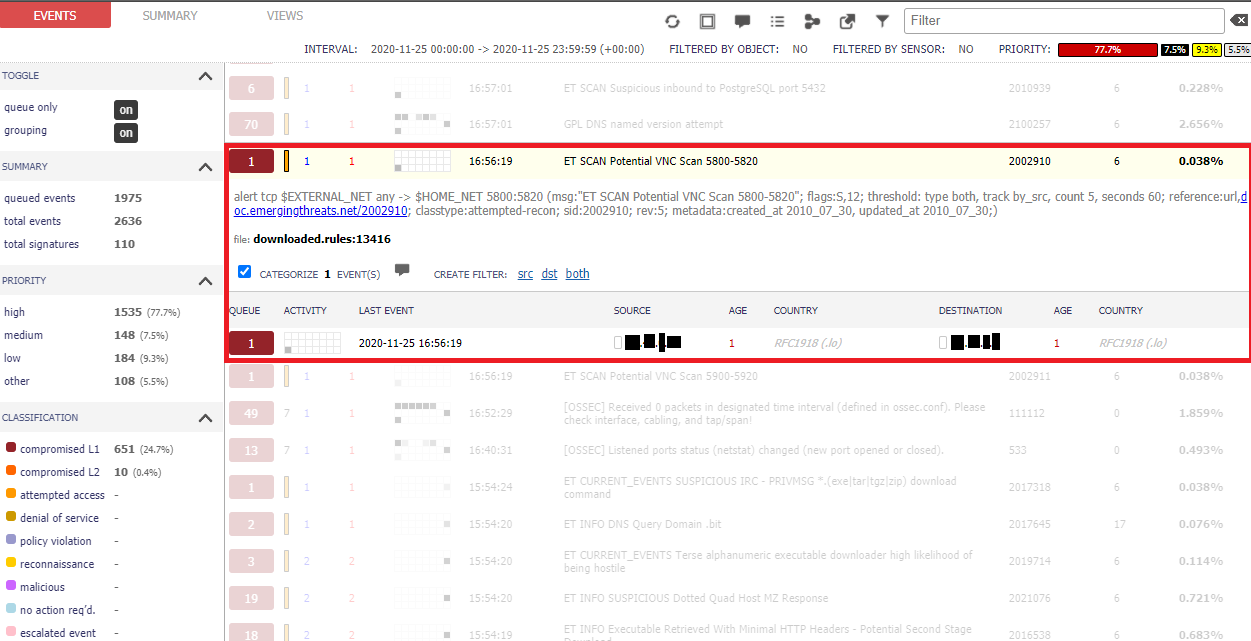
\includegraphics[width=1\textwidth]{./iteracion_3_imagenes/squert_ataque_vnc_L2-EDITADO.png}
        \caption{Incidente de reconocimiento en Squert. Prioridad nivel 2}
        \label{fig:squert-L2}
    \end{figure}
    \begin{figure}[H]
        \centering
        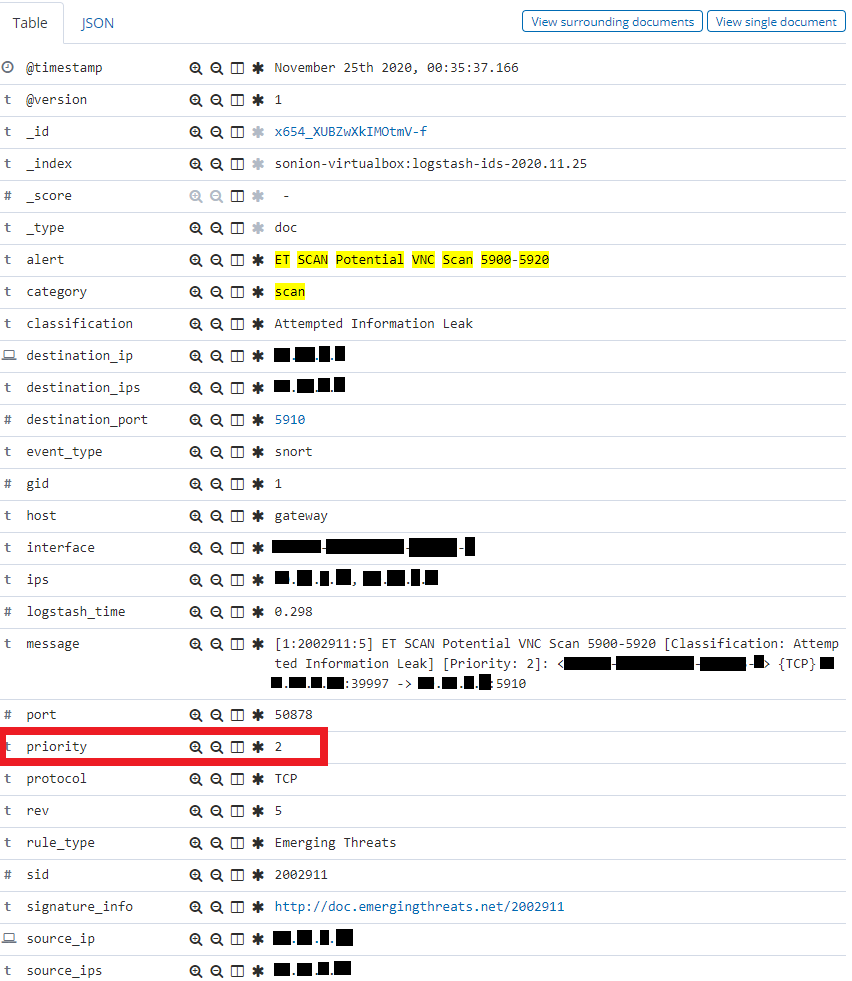
\includegraphics[width=1\textwidth]{./iteracion_3_imagenes/kibana_ataques_L2_1EDITADO.png}
        \caption{Incidente de reconocimiento en Kibana. Prioridad nivel 2}
        \label{fig:Kibana-L2}
    \end{figure}
    \FloatBarrier
    Se modificó el archivo \textbf{classification.config} para elevar el nivel de prioridad de los eventos asociados a la categoría “\textit{attempted-recon}”, que pasó del nivel 2 al nivel 1. Posteriormente se reiniciaron los sensores mediante el comando “\textit{so-sensor-restart}” y se procedió a comprobar los resultados de la modificación. Se repitió el ataque de reconocimiento y se pudo observar en las Figuras \ref{fig:squert-L1} y \ref{fig:kibana-L1} que Squert detectaba el ataque con prioridad 1 (barra vertical roja) y en Kibana se observó que el campo “priority” contenía el valor 1. Con esto se da por cumplido el requerimiento funcional 5.
    
    \begin{figure}[H]
        \centering
        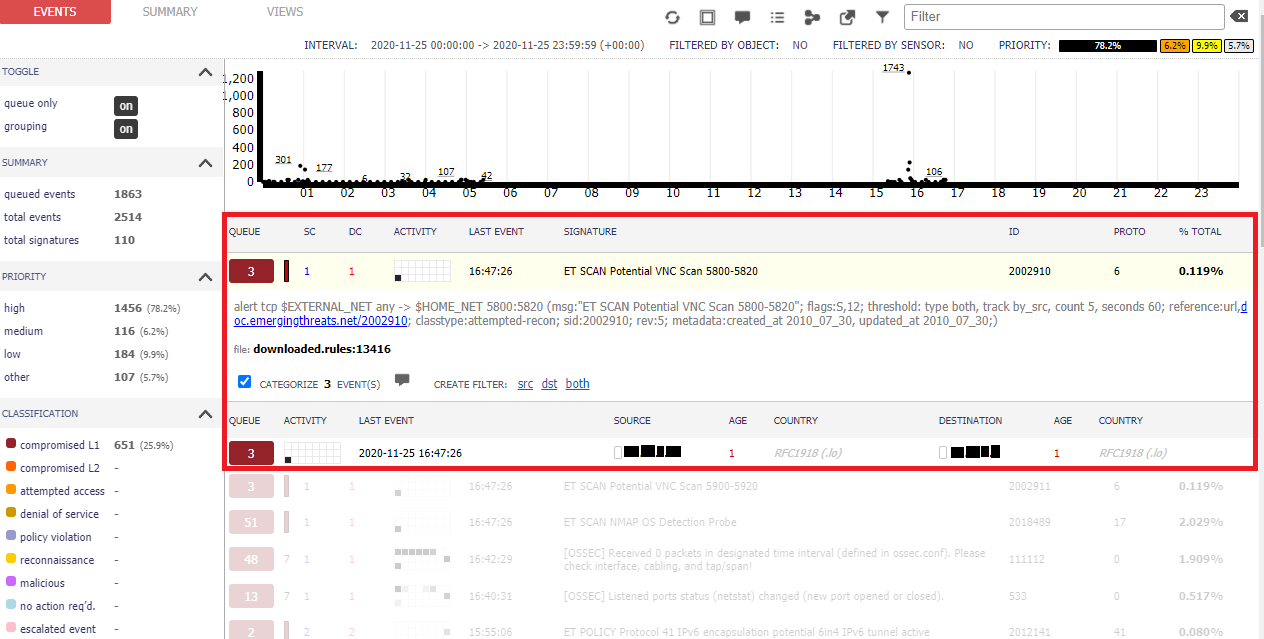
\includegraphics[width=1\textwidth]{./iteracion_3_imagenes/squert_ataque_vnc_L1-EDITADO.png}
        \caption{Incidente de reconocimiento en Squert. Nivel 1}
        \label{fig:squert-L1}
    \end{figure}
    \begin{figure}[H]
        \centering
        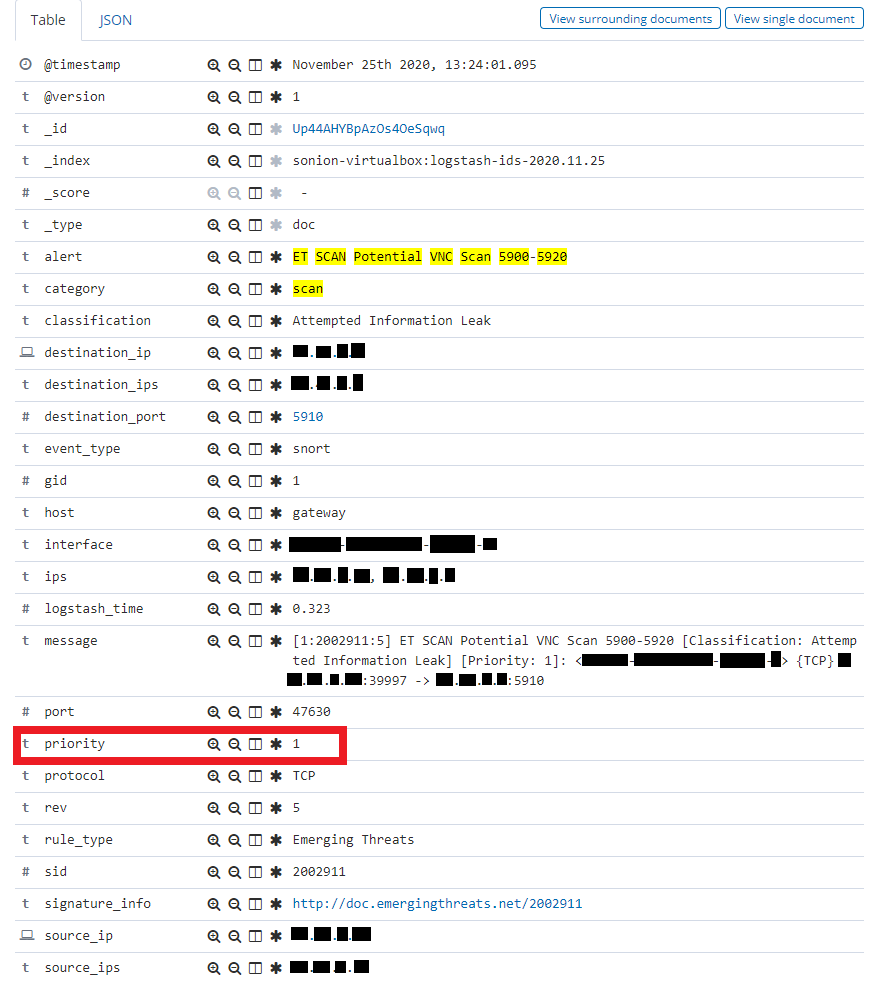
\includegraphics[width=1\textwidth]{./iteracion_3_imagenes/kibana_ataques_L2_2-EDITADO.png}
        \caption{Incidente de reconocimiento en Kibana. Nivel 1}
        \label{fig:kibana-L1}
    \end{figure}
    
    \end{section}

    \end{section}